\documentclass{standalone}
\usepackage{tikz}

\begin{document}

\begin{tikzpicture}
  \node[draw,inner sep=0pt] (a1) at (0,0) {
    \begin{tikzpicture}[scale=.5]
      \draw (-2,-1) rectangle (2,1);
      \foreach \i/\j [count=\xi from -1] in {b_2/b_2,b_1/b_1} {
        \node (\i) at (\xi,0) {$\j$};
      }
      \foreach \i/\j [count=\yi from -1] in {b_4/b_4,b_3/b_3} {
        \node (\i) at (\yi,.5) {$\j$};
      }
    \end{tikzpicture}
  };
  \node at (a1.south west) {$B_2 = \operatorname{Hex}(b_1 b_2 b_3 b_4)$};

  \node[draw,inner sep=0pt] (a2) at (6,0) {
    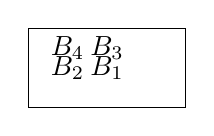
\begin{tikzpicture}[scale=.5]
      \draw (-2,-1) rectangle (2,1);
      \foreach \i/\j [count=\xi from -1] in {B_2/B_2,B_1/B_1} {
        \node (\i) at (\xi,0) {$\j$};
      }
      \foreach \i/\j [count=\yi from -1] in {B_4/B_4,B_3/B_3} {
        \node (\i) at (\yi,.5) {$\j$};
      }
    \end{tikzpicture}
  };
  \node at (a2.south west) {$B_4 = B_1^1 B_2^2 B_3^3 B_4^4$};

  \node[draw,inner sep=0pt] (a3) at (12,0) {
    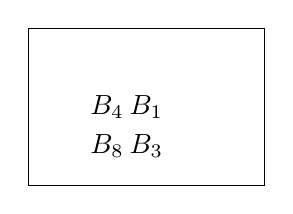
\begin{tikzpicture}[scale=.5]
      \draw (-3,-2) rectangle (3,2);
      \foreach \i/\j [count=\xi from -1] in {B_4/B_4,B_1/B_1} {
        \node (\i) at (\xi,0) {$\j$};
      }
      \foreach \i/\j [count=\yi from -1] in {B_8/B_8,B_3/B_3} {
        \node (\i) at (\yi,-1) {$\j$};
      }
    \end{tikzpicture}
  };
  \node at (a3.south west) {$B_8 = B_1^1 B_2^2 B_3^3 B_4^4$};
\end{tikzpicture}

\end{document}